\section{GraphRule}



Die neue Regel GraphRule mit ihrer Regelmenge RS-Graph wurde von \cite{shanbhag2014optimizing} entwickelt und getestet. Die neue Regel wurde implementiert, da der Volcano Optimier, der für seine Anpassungsfähigkeit verantwortlich ist und daher als Vorbild für Pyro(J) gewählt wurde, zwar für seine Anpassungsfähigkeit jedoch nicht für seine Geschwindigkeit bekannt ist. Die Join-Reihenfolge wird bei diesen Systemen durch Regelmengen wie das von Pellenkoft bestimmt. Die Enumeration von Plänen mit Hilfe von Transformationsregeln ist verglichen mit state-of-the-art Enumeratoren ineffizient. Ein Beispiel für einen solchen state-of-the-art Enumerator ist \texttt{MinCutConservative}. Dieses Verfahren ist zwar erheblich effizienter, jedoch nicht im selben Maß erweiterbar. Um die Vorteile beider Systeme zu vereinen, wurde von \cite{shanbhag2014optimizing} eine neue Regel mit dem Titel GraphRule entwickelt. Diese Regel ist die einzige Regel der Regelmenge RS-Graph. Die neue Regelmenge ist keine Erweiterung im eigentlichen Sinne. Sie ersetzt die bisherigen Regelmengen.

Im Folgenden werden die Grundlagen der Regel erläutert, ihr Vorgehen vorgestellt und die Geschwindigkeitsverbesserungen, die gemessen werden konnten behandelt.

\subsection{Top-Down-Enumeration}

Um mit der neuen Regel GraphRule zu starten, muss zuerst auf alternative Ansätze zur kreuzproduktfreien Erzeugung von Plänen eingegangen werden. Es gibt zwei unterschiedliche Ansätze: Top-Down-Join-Enumeration mit Memorizing und Bottom-Up-Join-Enumeration mit Dynamic Programming. Ein Bottom-Up-Enumerator ist DPccp, der von \cite{moerkotte2006analysis} entwickelt wurde. Der Nachteil dieser Enumeratoren ist, dass die Generierten Bäume nicht beschnitten werden können, was bei Top-Down-Join-Enumeratoren der Fall ist.

Der von \cite{dehaan2007optimal} entwickelte Algorithmus TDMinCutLazy ist der erste effiziente Top-Down-Join-Enumerator. Der alternative Top-Down Algorithmus TDMinCutBranch, der fast an die Geschwindigkeit von DPccp heranreichte, wurde in der Folge von \cite{fender2011new} präsentiert. Im Gegensatz zu TDMinCutLazy, der auch Kreuzprodukte generierte, nutzte TDMinCutBranch eine Graphen-basierte Enumerationsstrategie, die nur kreuzproduktfreie Pläne erzeugt.  Auf Basis dieses Algorithmus wurde der weiter verbesserte Algorithmus TDMinCutConservative von \cite{fender2012effective} vorgestellt. Der Algorithmus ist leichter zu implementieren und noch schneller als sein Vorgänger. 



\subsubsection{Generische Top-Down-Enumeration}

Die Funktionsweise eines generischen Top-Down-Enumerators lässt sich am einfachsten an einem Codebeispiel nachvollziehen. Hierzu ist es notwendig die folgende Notation  zu verstehen:

\begin{itemize}
\item $E$: Kanten zwischen Knoten
\item $V$: Knoten eines Baums
\item $G$: Graph von Kanten und Knoten ( $G = (V,E)$ )
\item $R$: Relationen, die auch als Knoten dargestellt werden können
\end{itemize}


\begin{figure}[ht]
  \centering
  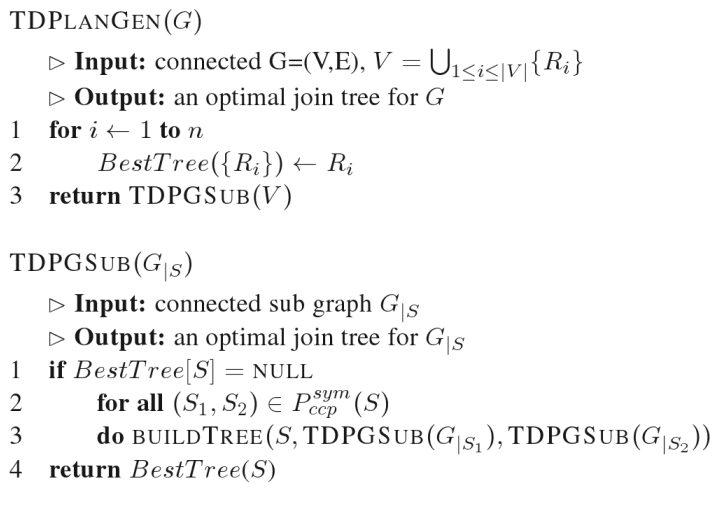
\includegraphics[scale=0.4]{03_Regeln/00_media/TDPlanGen.png}
  \caption{PseudoCode: TDPlanGen}
  \label{TDPlanGen}
\end{figure}


Wie in Abb. \ref{TDPlanGen} zu erkennen, beginnt die Top-Down-Enumeration mit einem Aufruf der Methode \texttt{TDPlanGen(G)}. Ihr wird ein Graph übergeben. Der Graph besteht aus Knoten und Kanten. Das Ergebnis der Methode ist ein optimaler Join-Tree.

Zuerst wird wie in Zeile 2 zu sehen, für jede Relation - sie sind nicht weiter trennbar, daher können keine Alternativen gebildet werden - die beste Variante für ihren jeweiligen Knoten festgelegt. Hierauf wird die Methode \texttt{TDGPSub(V)} aufgerufen. Es wird der gesamte Graph übergeben.


Die Methode \texttt{TDPGSub} prüft zuerst, ob für einen zu untersuchenden Subgraphen bereits ein bester Plan existiert. Ist dies der Fall wird abgebrochen. Falls noch kein bester Plan ermittelt wurde, werden aus dem Subgraphen \texttt{S} durch eine Partitionierungsmethode - sie wird später erläutert - Paare von Subgraphen erzeugt. Für jedes Paar wird ein neuer Baum erstellt. Aus der Menge der neuen Bäume wird dann der beste ausgewählt und ausgegeben. 


\begin{figure}[ht]
  \centering
  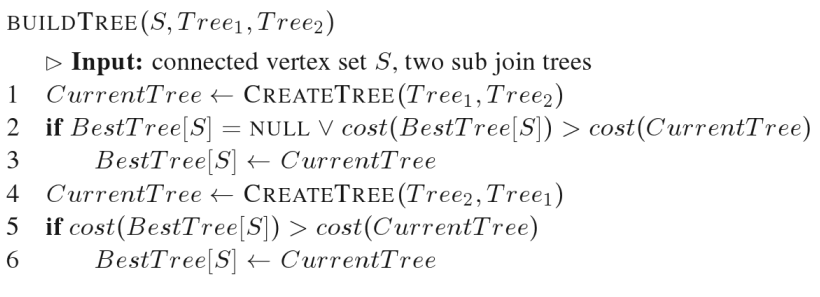
\includegraphics[scale=0.4]{03_Regeln/00_media/BuildTree.png}
  \caption{PseudoCode: BuildTree}
  \label{BuildTree}
\end{figure}

In der Methode \texttt{BuildTree} (vgl. Abb. \ref{BuildTree}) wird aus zwei Teilbäumen zuerst ein neuer Baum gebildet. Falls die Kosten dieses neuen Baums niedriger für den Subgraphen \texttt{S} sind,  als alle bisher bekannten Pläne, wird der neue Plan als Optimaler Plan gespeichert. Nachdem diese Methode für alle Partitionen eines Subgraphen durchlaufen ist, ist sichergestellt, dass die Kosten für jeden alternativen Graphen verglichen wurden und auch der beste alternative Plan ausgewählt wurde.

\begin{figure}[ht]
  \centering
  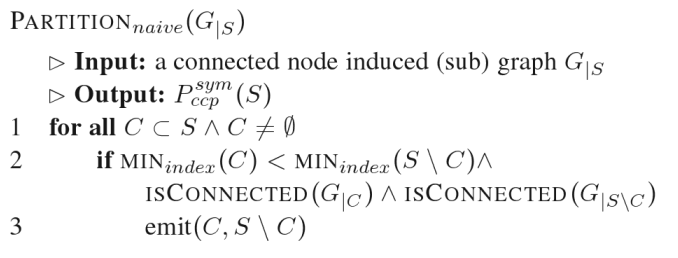
\includegraphics[scale=0.4]{03_Regeln/00_media/Partition.png}
  \caption{PseudoCode: Partition}
  \label{Partition}
\end{figure}


Die Paritionierung eines Graphen in Subgraphen geschieht mit der Methode \texttt{Partition} (vgl. Abb. \ref{Partition}). Aus dem Ausgangsgraphen wird zuerst ein Teilstück \texttt{C} herausgeschnitten. Dieser Teil ist Bestandteil des Subgraphen \texttt{S}. Für jedes Teilstück wird geprüft, ob es mit dem Graphen \texttt{S} verbunden ist. Ist dies der Fall, wird ein neues Paar an Subgraphen erstellt. Es besteht aus \texttt{C} und  \texttt{S\textbackslash C}. \texttt{S\textbackslash C} und \texttt{C} ergeben so gemeinsam \texttt{S}.


\subsubsection{Partitionierung mit MinCutConservative}

\begin{figure}[ht]
  \centering
  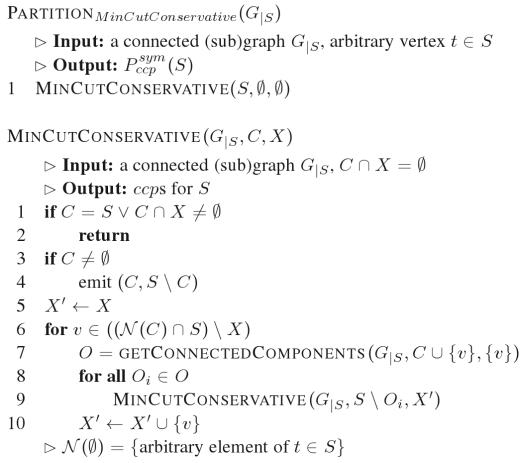
\includegraphics[scale=0.5]{03_Regeln/00_media/MinCutConservative.png}
  \caption{PseudoCode: MinCutConservative}
  \label{MinCutConservative}
\end{figure}

\texttt{MinCutConservative} ist eine konkrete Implementierung eines Partitionierungsalgorithmus, der auch für GraphRule zum Einsatz kommt. In bestimmten Szearios wie sternförmigen Abfragen, kann die Generierung von jeder Teilmenge \texttt{T} eines Subgraphen \texttt{S} exponentiellen Overhead erzeugen, da die meisten komplementären Bäume \texttt{S\textbackslash C} nicht miteinander verbunden sind und somit keine validen, kreuzprduktfreien Teilbäume entstehen. Um zu vermeiden, dass ein komplementärer Baum entsteht, der nicht verbunden ist, wird in diesem konservativen Ansatz nur ein \texttt{C} gewählt, dessen Komplement auch verbunden ist. 







\subsection{Transformationsregel: GraphRule}

Die GraphRule \cite{shanbhag2014optimizing} bedient sich der zuvor vorgestellten Implementierung von Top-Down-Enumeratoren. Die Regel, um kompatibel zu anderen Regeln und den Regelmengen zu sein, verwendet das selbe Interface wie andere Regeln: \texttt{GraphRule($\Join, A, B, parent$)}.  Ziel der Regel ist es alle möglichen Transformationen für einen initialen Anfragegraphen mit nur einem Aufruf auszugeben. 

\begin{figure}[ht]
  \centering
  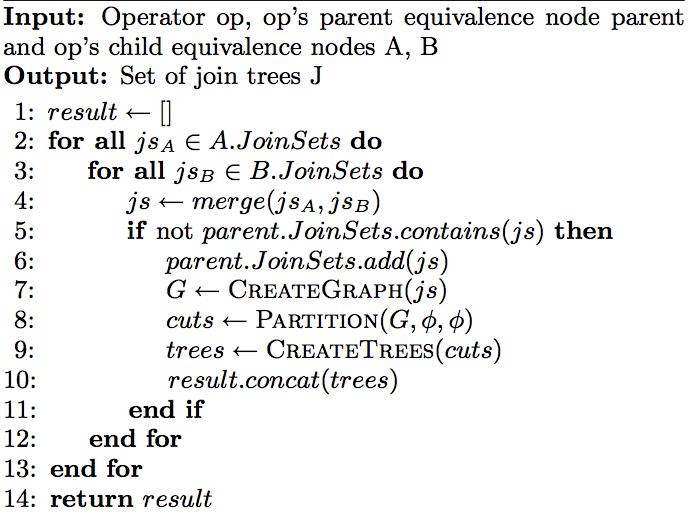
\includegraphics[scale=0.4]{03_Regeln/00_media/GraphRule.png}
  \caption{PseudoCode: GraphRule}
  \label{GraphRule}
\end{figure}

Im Vergleich zu Abb. \ref{TDPlanGen} fällt in Abb. \ref{GraphRule} auf, dass JoinSets und eine neue \texttt{merge}-Methode verwendet wird. Ebenfalls kommt anstatt von \texttt{BestPlan} \texttt{CreateGraph} zum Einsatz. Ein weiterer grundlegender Unterschied ist, dass anstatt von Knoten, die Relationen repräsentieren, Äquivalenzklassen zum Einsatz kommen.

Join-Sets bezeichnen für einen Äquivalenzknoten $E$ ein Paar von $J = (V,P)$, wobei $V$ eine Menge von Äquivalenzknoten ist und $P$ eine Menge von Prädikaten zwischen diese Knoten.  Damit ein Join-Set ähnlich zu einem Graphen, wie er bei der Top-Down-Enumeration beschrieben wurde. Der einzige Unterschied besteht darin, dass eine Äquivalenzklasse mehrere dieser Paare an Kanten und Knoten beinhalten kann.

Wie in der Regel zu sehen, wird eine linke Äquivalenzklasse $A$ und eine rechte Äquivalenzklasse $B$ übergeben. Aus jedem Join-Set der linken und rechten Seite wird in Zeile 4 ein neues Join-Set gebildet. Falls dieses neue Join-Set noch nicht bekannt ist, kann in Zeile 5 fortgefahren werden.  Mit der Prüfung wird sichergestellt, dass eine Kombination des linken und rechten Join-Sets nicht mehrfach bearbeitet wird. Aus den Join-Sets muss in Zeile 7 eine verarbeitbare Form für den Partitionierungsalgorithmus generiert werden. Hier wird aus dem Join-Set ein Graph gebildet. Dieser Graph wird durch MinCutConservative oder einen anderen Partitionierungsalgorithmus zerteilt. Aus den einzelnen Stücken wird ein neuer Baum zusammengesetzt. Bei der Zusammensetzung werden Äquivalenzklassen und Planknoten verwendet, anstatt Knoten und Kanten. So entsteht wieder eine Form, die kompatibel mit dem Regel-Interface ist. Eine Berechnung des besten Plans, wie es bei \texttt{BuildTree} vorgesehen ist, findet nicht statt.



\subsection{Vollständigkeit von GraphRule}
Die Vollständigkeit der GraphRule und damit der Regelmenge RS-Graph wird von \cite{shanbhag2014optimizing} dadurch festgestellt, dass der zu Grunde liegende Algorithmus \texttt{Min\-Cut\-Conserva\-tive} aus einem gegebenen Join-Graphen $G = (V,E)$. Es wird festgestellt, dass \cite{fender2012effective} bewiesen hat, dass \texttt{Min\-Cut\-Conservative} alle möglichen $(S_1, S_2)$, die durch ein Join-Prädikat verbunden sind, erzeugen kann. Unter der Vorraussetzung, dass der Algorithmus zur Partitionierung des Graphen korrekt implementiert ist, lässt sich aus diesen Teilstücken mit Hilfe der Methode \texttt{createGraph} ein neuer Plan zusammensetzen. Diese Methode orientiert sich an der Methode \texttt{BestPlan}.



